\documentclass[12pt]{article}
\usepackage[paper=letterpaper,margin=2cm]{geometry}
\usepackage{amsmath}
\usepackage{amssymb}
\usepackage{amsfonts}
\usepackage{newtxtext, newtxmath}
\usepackage{enumitem}
\usepackage{titling}
\usepackage{svg}
\usepackage{xcolor}
\usepackage{mathtools}
\usepackage{listings}
\usepackage[colorlinks=true]{hyperref}

\setlength{\droptitle}{-6em}

\definecolor{codegreen}{rgb}{0,0.6,0}
\definecolor{codegray}{rgb}{0.5,0.5,0.5}
\definecolor{codepurple}{rgb}{0.58,0,0.82}
\definecolor{backcolour}{rgb}{0.95,0.95,0.92}

\lstdefinestyle{mystyle}{
    commentstyle=\color{codegreen},
    keywordstyle=\color{magenta},
    numberstyle=\tiny\color{codegray},
    stringstyle=\color{codepurple},
    basicstyle=\ttfamily\footnotesize,
    breakatwhitespace=false,
    breaklines=true,
    captionpos=b,
    keepspaces=true,
    numbers=left,
    numbersep=5pt,
    showspaces=false,
    showstringspaces=false,
    showtabs=false,
    tabsize=2
}

\lstset{style=mystyle}
% https://stackoverflow.com/questions/1116266/listings-in-latex-with-utf-8-or-at-least-german-umlauts
\lstset{%
        inputencoding=utf8,
        extendedchars=true,
        literate=%
        {é}{{\'{e}}}1
        {è}{{\`{e}}}1
        {ê}{{\^{e}}}1
        {ë}{{\¨{e}}}1
        {É}{{\'{E}}}1
        {Ê}{{\^{E}}}1
        {û}{{\^{u}}}1
        {ù}{{\`{u}}}1
        {ú}{{\'{u}}}1
        {â}{{\^{a}}}1
        {à}{{\`{a}}}1
        {á}{{\'{a}}}1
        {ã}{{\~{a}}}1
        {Á}{{\'{A}}}1
        {Â}{{\^{A}}}1
        {Ã}{{\~{A}}}1
        {ç}{{\c{c}}}1
        {Ç}{{\c{C}}}1
        {õ}{{\~{o}}}1
        {ó}{{\'{o}}}1
        {ô}{{\^{o}}}1
        {Õ}{{\~{O}}}1
        {Ó}{{\'{O}}}1
        {Ô}{{\^{O}}}1
        {î}{{\^{i}}}1
        {Î}{{\^{I}}}1
        {í}{{\'{i}}}1
        {Í}{{\~{Í}}}1
}


\title{\large{Aprendizagem 2022}\vskip 0.2cm Homework I -- Group 019\vskip 0.2cm Diogo Gaspar 99207, Rafael Oliveira 99311}
\date{}
\begin{document}
\maketitle
\center\large{\vskip -2.5cm\textbf{Part I}: Pen and paper}
\begin{enumerate}[leftmargin=\labelsep]
\item \textbf{Draw the training confusion matrix.}

After consulting the decision tree described in the question's statement,
we can assert that its confusion matrix is the following:

\begin{figure}[htpb]
  \centering
  \includesvg{../assets/hw1-1.1.svg}
  \caption{Confusion Matrix}
\end{figure}

\item \textbf{Identify the training F1 after a post-pruning of the given tree under a maximum depth of 1.}

\begin{figure}[htpb]
\centering
\includesvg{../assets/hw1-1.2.svg}
\caption{Post-pruning confusion matrix}
\end{figure}

We know that:

$$
d = 1: \quad F_1 = \frac{2 * \text{Precision} * \text{Sensitivity}}{\text{Precision} + \text{Sensitivity}}
$$

Therefore, we must calculate the associated precision and sensitivity as follows:

$$
\text{Sensitivity} = \frac{TP}{TP + FN} = \frac{5}{5 + 6} = \frac{5}{11}
$$

$$
\text{Precision} = \frac{TP}{TP + FP}= \frac{5}{5 + 2} = \frac{5}{7}
$$

We can, now, calculate the F1 score:

$$
d = 1: \quad F_1 = \frac{2 * \frac{5}{7} * \frac{5}{11}}{\frac{5}{7} + \frac{5}{11}} = \frac{5}{9}
$$

\item \textbf{Identify two different reasons as to why the left tree path was not further decomposed.}

We can find multiple reasons for the left-most tree path not being further decomposed.

The first, perhaps most obvious reason is that we want to \textbf{avoid overfitting} the
tree to the training data: given a threshold of $\frac{5}{7}$, it's already possible
to make a very fair, general assessment about all instances that fall under the $y_1 = A$
condition (asserting they fall onto the $P$ label). It's obviously not guaranteed
that not further decomposing the tree will lead to a better labeling come testing time,
but generally speaking it ends up being a good practice to avoid overfitting.

Related to the overfitting idea, there also aren't many instances (only 7) in the
left path, which makes it so that further decomposing that path doesn't change
the classification error by much (if at all), while also adding unnecessary
complexity to the tree - therefore, it's \textbf{not likely} that there will be a significant
\textbf{entropy reduction} by further decomposing the left-most tree path.

\item \textbf{Compute the information gain of variable y1.}

We know that:

\begin{equation}
  \operatorname{IG}(y_{out} \mid y_1) = \textcolor{teal}{\operatorname{H}(y_{out})} - \textcolor{violet}{\operatorname{H}(y_{out} \mid y_1)}
\end{equation}

\begin{equation}
  \operatorname{H}(Y) = -\sum_{y \in Y} p(y) \log_2 p(y)
\end{equation}

Considering $y_{out}$ as our \textit{output variable}, with possible values $P$ or $N$,
we'll be able to see that:

\begin{equation}
  \operatorname{H}(y_{out}) = \textcolor{teal}{(- \frac{11}{20} \log_2 \frac{11}{20} - \frac{9}{20} \log_2 \frac{9}{20})}
\end{equation}

\begin{equation}
  \operatorname{H}(y_{out} \mid y_1) = \textcolor{violet}{\left[\frac{7}{20}(- {\frac{5}{7}} \log_2 \frac{5}{7} - \frac{2}{7} \log_2 \frac{2}{7}) + \frac{13}{20}(- \frac{6}{13} \log_2 \frac{6}{13} - \frac{7}{13} \log_2 \frac{7}{13})\right]}
\end{equation}

We have, therefore:

$$
\operatorname{IG}(y_{out} \mid y_1) = 0.04345941113
$$

\end{enumerate}

\center\large{\textbf{Part II}: Programming}

\begin{enumerate}[leftmargin=\labelsep,resume]
\item \textbf{Using \texttt{sklearn}, apply a stratified 70-30 training-testing split with a fixed seed (\texttt{random\_state=1}), and assess in a single plot the training and testing accuracies of a decision tree with no depth limits (and remaining default behavior) for a varying number of selected features in \{5,10,40,100,250,700\}. Feature selection should be performed before decision tree learning considering the discriminative power of the input variables according to mutual information criterion (\texttt{mutual\_info\_classif}).}

\begin{figure}[htpb]
  \centering
  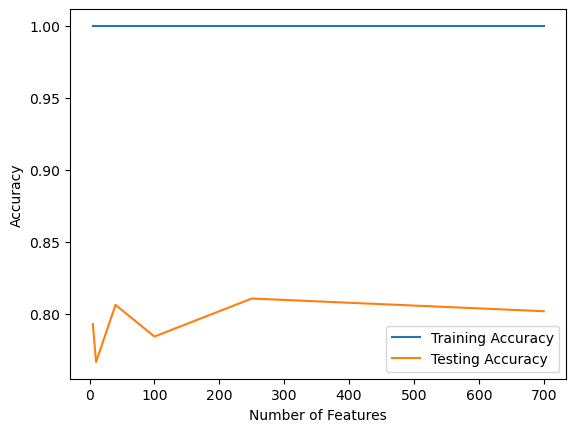
\includegraphics[width=0.8\textwidth]{../assets/hw1-2.1.png}
  \caption{Training and Testing Accuracy vs. Number of Features}
\end{figure}

The code utilized to generate the plot is present in the report's appendix.

\item \textbf{Why is training accuracy persistently 1? Critically analyze the gathered results.}

Since the decision tree has no depth-limit associated, the worst-case scenario sees the tree
holding exactly one leaf per training sample - leading to there always being a "correct path" in the tree for a given observation - and thus the training accuracy is always 1, for any train-test split of the dataset.

The testing accuracy isn't necessarily 1, of course, just like it can be seen in the plot shown above: in the vast majority of cases, the testing set will hold samples which differ from all seen in the training set, effectively evicting the "guarantee" of a correct guess from the decision tree. It can, of course, still take a correct guess (with that being our goal), but it's not guaranteed.

\end{enumerate}

\large{\textbf{Appendix}\vskip 0.3cm}

Code utilized in the first question of the programming section shown in the pages below:

\lstinputlisting[language=Python]{code.py}

\end{document}
